\chapter{Discussions des résultats et travaux futurs}



\begin{figure*}[!h]

   \centering
   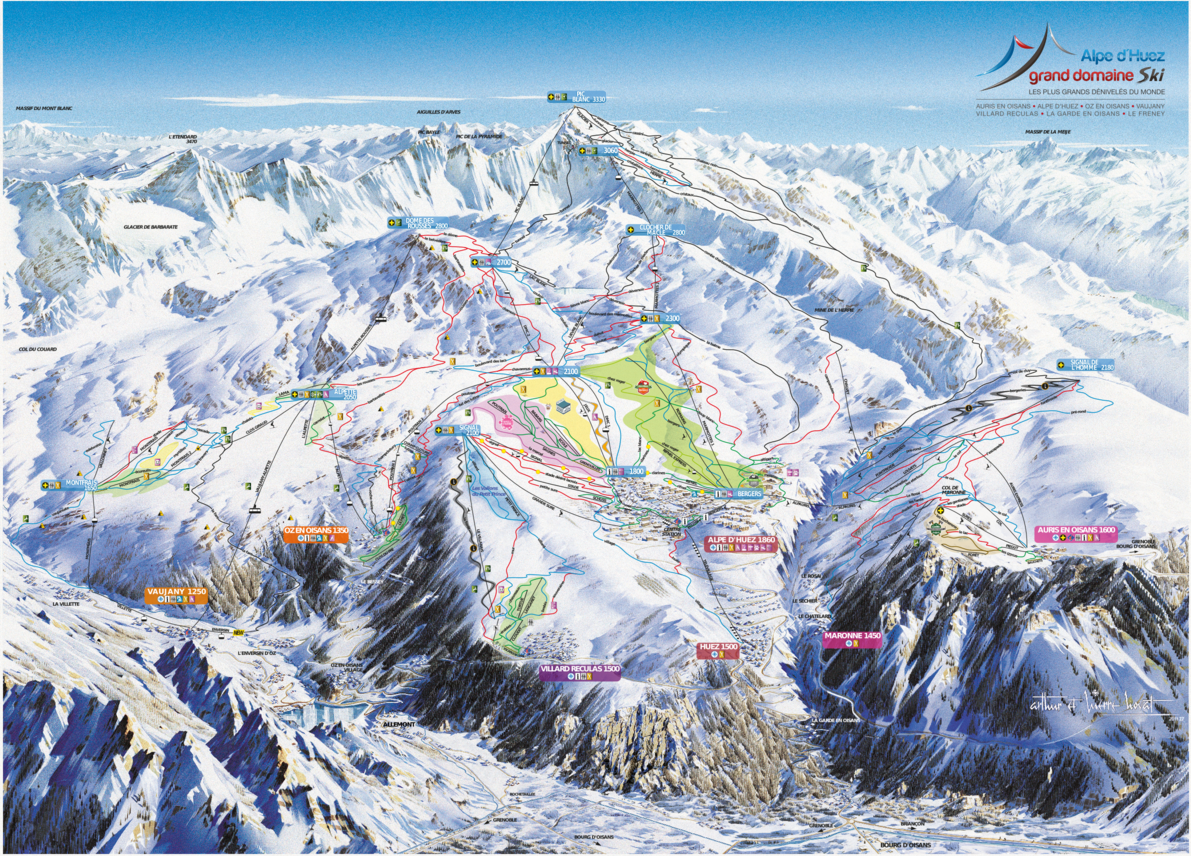
\includegraphics[width=1.0\linewidth]{novat/AlpeHuez_pistes.png}
   \caption{Plan des pistes de l'alpe d'Huez par Arthur et Pierre Novat.}
\end{figure*}














Notre méthode permet de mettre en valeur toutes les aspérités d'un terrain en faisant un rendu expressif des ombres. Les résultats sont convaincants cependant la méthode est incomplète et il manque une couche "artistique" pour donner un vrai aspect "Novat" à notre rendu. 
\section{L'ombrage expressif}
	L'ombrage est notre principale contribution au rendu de panorama du style de Pierre Novat. Cependant notre méthode n'est pas encore assez générique. En effet, notre méthode se base uniquement sur une pyramide Laplacienne à deux échelles (Fig. \ref{fig:pyramide}), l'une floue, l'autre détaillée (ce qui suffit pour des cartes hauteur avec un pas de 25m mais qui est très insuffisant pour des cartes avec un pas de 1m). Il faudrait pouvoir la généraliser en pouvant faire un nombre arbitraire d’échelles comme dans le papier d'\textit{exagerated shading}  \cite{rusinkiewicz2006exaggerated}. La question sera alors de savoir comment les fusionner et qu'est-ce que ça signifie de faire un ombrage intermédiaire.  En effet notre méthode utilisant une fonction de type "Overlay", qui ne permet pas de s’étendre facilement à $N$ paramètres. La solution naïve serait de fusionner deux par deux les cartes en remontant (ou descendant les échelles) mais cela voudrait dire que la première échelle (ou la dernière) serait la plus importante ce qui ne correspondrait pas forcément à l'effet attendu. Ensuite nous pourrions changer la fonction de fusion. Nous pensons effectivement que notre fonction actuelle est améliorable. Le problème est que le choix de la fonction de fusion n'est pas un choix qui ne sert qu'à optimiser la lecture. C'est un aussi choix qui influence le style du panorama en augmentant ou diminuant le contraste des certaines ombres (par exemple, notre méthode augmente le contraste de l'ombrage de la partie détaillée au détriment de l'ombrage de la partie floutée (Fig. \ref{fig:comparaisonFusion}). Enfin malgré le fait que nous souhaitons faire un rendu style "Novat", une validation plus formelle de notre méthode d'ombrage devrait êtes faite a l'aide des gradients par exemple. 

D'un autre coté, il y a les ombres portées. Notre méthode inclue des ombres portées multi-échelle mais à la lecture des panoramas de Pierre Novat, il possible qu'un calcul d'ombre portée à une seule échelle suffise (sur les montagnes les plus importantes). Ensuite dans notre méthode, il y a trois points à améliorer. Le premier est l'ajustement local du vecteur lumière. Si nous voulons avoir de l'ombre uniquement sur les zones importantes, il faudrait ajuster la hauteur de ce vecteur, par exemple à la pente. Le second est la forme de ces ombres portées. Nous n'avons pas exploité tout ce que pouvait offrir la morphologie mathématique et une idée qui pourrait être testée est de faire un élément structurant avec une forme orientée dans le sens de la lumière plutôt qu'un simple carré et adapté à la résolution de la carte. Enfin le troisième point est la fusion entre ombres portées et ombrage. Dans notre méthode nous fusionnons les ombres portées avec l'ombrage puis nous ajoutons une couche de couleur. Seulement Arthur Novat nous indique que l'ombrage et les ombres portées sont deux couches de couleur qu'il applique l'une sur l'autre. 

Une fois l'ombrage fait nous avons essayé de colorier notre résultat afin d'avoir un rendu plus proche des panoramas du style de Novat. Nous avons essayé plusieurs méthodes : aquarelle, dégradé de couleur, \textit{cel-shading} (Fig \ref{fig:colorOmbre}. Après avoir les avoir montrées à Arthur Novat, il nous a dit que l’aquarelle ressemblait au $1^{er}$ calque qu'il faisait.  De plus il nous a indiqué que la couleur n'était pas que fonction de l'ombrage mais aussi de l'altitude. Ainsi une idée serait d'utiliser un \textit{xToon} \cite{barla2006x} pour avoir une rampe de couleur à deux dimensions, l'une contrôlée par l'ombrage, l'autre par l'altitude. 

Enfin une partie qui sort de notre contribution mais qui est importante pour la suite est l'aspect artistique qu'il est nécessaire d'ajouter pour donner à l'ombrage et aux ombres portées un rendu plus proche du style Novat. En effet  il faudrait augmenter le contraste dans le faible relief et au contraire le baisser dans le haut relief. "Cela sert à donner de la cohérence" nous dit Arthur Novat. De plus il faut modifier la quantité de relief selon la pente : "plus la zone est pentue, plus le relief est dense" tout en empêchant "que ce soit trop vertigineux". De plus les fonds des vallées devraient plus ressortir. Enfin le dessin des ombres devrait être plus complexe. Il faudrait qu'elles soit dégradées avec uniquement le bord de l'ombre qui soit vraiment sombre, et ajouter de l'occlusion ambiante et de l'inter-réflexion entre les montagnes.

\section{Style Novat}
	Une fois la question de l'ombrage résolue, il restera encore beaucoup de travail pour avoir un vrai rendu de panorama style Novat. Dans un premier temps, il faudrait lier notre méthode d'ombrage à la déformation de montagne fait au LIG pour avoir un vrai aperçu de ce que pourrait donner un panorama style Novat fait de manière "automatique".

Ensuite, il faut rajouter les élément décoratifs : rochers, arbres, maisons et routes. Mais chaque élément demande une attention particulière si nous voulions rester fidèle au style. Chaque élément pose deux questions : où le placer et comment le dessiner. Les rochers par exemple peuvent être placés quand la pente devient trop forte et dessinés à l'aide d'une texture procédurale  \cite{perlin2002improving}  ou des textures définies par l'utilisateur \cite{loi2015programmable}. Même constat pour les arbres qui peuvent être dessinés de la même manière mais il faudrait savoir où les placer (en utilisant d'autres carte de l'IGN par exemple) et comment les placer, car ils sont alignés à la pente. De plus ils possèdent une ombre non négligeable qu'il faudrait prendre en compte dans notre méthode d'illumination. Ensuite pour les maisons c'est encore une autre question car elles représentent assez fidèlement les villages, il faut donc arriver à extraire leur forme de cartes ou de photos pour pouvoir les traduire dans un style Novat. De plus comme pour les sapins, il faut les intégrer à notre modèle d'illumination. Enfin les routes sont peut être un peu plus simples à faire, il faut juste leur donner un aspect continu et "creuser" la montagne là ou elles passent pour les faire ressortir. 

Enfin la dernière chose à faire est d'intégrer des niveaux de détails, c'est-à-dire faire en sorte que plus nous nous éloignons du point de vue, plus les détails s'effacent et plus nous avons un aspect générique. 


\section{Conclusion}
Dans ce rapport nous avons produit deux contributions : l'étude du style de Pierre Novat et le calcul d'un ombrage expressif. Notre rendu répond à la question de comment faire ressortir toutes les variations d'un terrain mais il reste incomplet dans le cadre d'un rendu de style Novat. La principale difficulté dans l'imitation d’œuvres artistiques est qu'il est difficile d'avoir un résultat convainquant dès le premier essai. Dans notre cas nous avons la chance, contrairement aux autres publication dans le même style \cite{bratkova2009artistic}\cite{brown2017real}, d'être en contact direct avec l'artiste et c'est grâce aux discussions avec Arthur Novat que nous avons pu avancer. Mais il est difficile pour lui d'exprimer d'un seul coup tous les algorithmes mentaux qui lui servent à créer ses œuvres. Ainsi il a besoin d'une première solution pour pouvoir dire ce qui manque et de plus en plus préciser ce qui se passe quand il produit ses œuvres. C'est parce que la solution proposée donne une bonne base de relief que nous avons pu collecter des éléments d'information qui permettront d'aller plus loin. Ainsi, ce sont ces échanges continuels qui permettront,  je l'espère, à terme de créer un rendu très proche des panoramas Pierre Novat. 

    